% Copyright 2004 by Till Tantau <tantau@users.sourceforge.net>.
%
% In principle, this file can be redistributed and/or modified under
% the terms of the GNU Public License, version 2.
%
% However, this file is supposed to be a template to be modified
% for your own needs. For this reason, if you use this file as a
% template and not specifically distribute it as part of a another
% package/program, I grant the extra permission to freely copy and
% modify this file as you see fit and even to delete this copyright
% notice. 

\documentclass{beamer}

% There are many different themes available for Beamer. A comprehensive
% list with examples is given here:
% http://deic.uab.es/~iblanes/beamer_gallery/index_by_theme.html
% You can uncomment the themes below if you would like to use a different
% one:
%\usetheme{AnnArbor}
%\usetheme{Antibes}
%\usetheme{Bergen}
%\usetheme{Berkeley}
%\usetheme{Berlin}
%\usetheme{Boadilla}
%\usetheme{boxes}
%\usetheme{CambridgeUS}
%\usetheme{Copenhagen}
%\usetheme{Darmstadt}
%\usetheme{default}
%\usetheme{Frankfurt}
%\usetheme{Goettingen}
%\usetheme{Hannover}
%\usetheme{Ilmenau}
%\usetheme{JuanLesPins}
%\usetheme{Luebeck}
\usetheme{Madrid}
%\usetheme{Malmoe}
%\usetheme{Marburg}
%\usetheme{Montpellier}
%\usetheme{PaloAlto}
%\usetheme{Pittsburgh}
%\usetheme{Rochester}
%\usetheme{Singapore}
%\usetheme{Szeged}
%\usetheme{Warsaw}

\title{XML Injection Mutation for Web Services Vulnerability Testing
	Based on SOAP Messages}

% A subtitle is optional and this may be deleted
%\subtitle{Optional Subtitle}

%\author{Bimal Varghese\inst{1} \and Simi Stephen\inst{2}}
\author{Bimal Varghese \and Simi Stephen}
% - Give the names in the same order as the appear in the paper.
% - Use the \inst{?} command only if the authors have different
%   affiliation.

\institute[FISAT ] % (optional, but mostly needed)
{
 % \inst{1}%
  Department of Computer Science and Engineering\\
  Federal Institute of Science and Technology\\
  Mookkannoor
%  \and
 % \inst{2}%
  }
% - Use the \inst command only if there are several affiliations.
% - Keep it simple, no one is interested in your street address.

\date{\today}
% - Either use conference name or its abbreviation.
% - Not really informative to the audience, more for people (including
%   yourself) who are reading the slides online

%\subject{Theoretical Computer Science}
% This is only inserted into the PDF information catalog. Can be left
% out. 

% If you have a file called "university-logo-filename.xxx", where xxx
% is a graphic format that can be processed by latex or pdflatex,
% resp., then you can add a logo as follows:

% \pgfdeclareimage[height=0.5cm]{university-logo}{university-logo-filename}
% \logo{\pgfuseimage{university-logo}}

% Delete this, if you do not want the table of contents to pop up at
% the beginning of each subsection:
\AtBeginSubsection[]
{
  \begin{frame}<beamer>{Introduction}
    \tableofcontents[currentsection,currentsubsection]
  \end{frame}
}

% Let's get started
\begin{document}

\begin{frame}
  \titlepage
\end{frame}

\begin{frame}{Outline}
  \tableofcontents
  % You might wish to add the option [pausesections]
\end{frame}

% Section and subsections will appear in the presentation overview
% and table of contents.
\section{Introduction}

\subsection{Web Service}

\begin{frame}{Web Service}% {Optional Subtitle}
  \begin{itemize}
  \item {
    Common way of implementing SOA.
  }
  \item {
    Widely used in the Internet.
  }
  \item {
  	Quality and Reliability of Web Service must be heavily tested.
  	}
  \end{itemize}
\end{frame}

\subsection{Vulnerability Testing of Web Service}

% You can reveal the parts of a slide one at a time
% with the \pause command:
\begin{frame}{Vulnerabilities in WS}
  \begin{itemize}
  \item {
    Multiple Components in WS
    \pause % The slide will pause after showing the first item
  }
  \begin{itemize}
  	\item WSDL \pause
  	\item SOAP \pause
  	\item XML \pause
  	\item UDDI \pause
  \end{itemize}
  \pause
  \item {   Vulnerability refers to flaws
  	in the service that threaten the security of the computer
  	system
    
  }
  \pause
  % You can also specify when the content should appear
  % by using <n->:
  \item<3-> {
    Some types of
    Web service vulnerability faults might not be effectively
    revealed by traditional testing approaches
  }

  \end{itemize}
\end{frame}

\section{Base Paper}

\subsection{Mutation Operators}


\begin{frame}{Mutation Operators}{}
	\begin{itemize}
		\item Testing based on SOAP message.
		\item An extended Regular Tree Grammar(RTG) model
			\begin{itemize}
				\item $ < $ E; N; DT; P; A; $n_{s} > $
				\item E :finite set of elements.
				\item N :finite set of non Terminals.
				\item DT :finite set of Data types.
				\item P :finite set of production rules.
				\item A :2 tuple $ <n,type> $
				\begin{enumerate}
					\item n :number of parameters.
					\item type: parameter type.
				\end{enumerate} 
			\end{itemize}
		\item A mutation operator is
		r= $ f (n_{1}, n_{2},... n_{i}) $ where f is a function, i $ \geq $1, each
		$ n_{1}, n_{2},... n_{i}\epsilon N$ and has an arbitrary data type and r outputs mutated $ n_{1},n_{2},..n_{i} $ with the same data type.
		
		
	\end{itemize}
\end{frame}

\subsection{Worst Input Mutation }
\begin{frame}{Mutation Operators}{}
	\begin{itemize}
		\item Regular Mutation
		\begin{itemize}
			\item Small modification of the legitimate input
		\end{itemize}
		\pause
		\item Worst Input Mutation
		\begin{itemize}
			\item Use Farthest neighbor sequence from the legitimate input.
		\end{itemize}		
	\end{itemize}
\end{frame}

\begin{frame}{Contd\dots}
	\begin{itemize}
	\item Many program faults result in failures manifesting in contiguous areas of the
	input domain.
	\item if previously executed test cases have not revealed a failure, new
	test cases should be as far from the already executed non-failure test cases as possible
	\item For Testing, a Web Service Vulnerability Testing System (WSVTS)  is created
\end{itemize}
	\begin{block}{Advantages}
		\begin{itemize}
			\item Have the greatest possible test coverage.
			\item Typical representation for triggering faults.
			\item Low redundancy.
		\end{itemize}
	\end{block}
	
\end{frame}

\section{Problem Definition}
\subsection{XML Injection}
\begin{frame}{XML Injection}{}
	\begin{itemize}
		\item XML is the default way by which web service communicates.
		\item Also used in storing data with dynamic tag values.
		\item Tampering an XML will compromise the security of the web service.
		\item One of the most serious xml vulnerability is the XML injection.
		\item Can compromise data and even the security of the entire system itself. 
	\end{itemize}
\end{frame}
\section{Current Work}
\subsection{Testing Tool}
\begin{frame}{Work Completed}{}
	\begin{itemize}
		\item Web service Testing Tool is Created.
		
		\item Tool is able to identify the available Method names, their parameters, types, and their return values from the wsdl file.
		\item It is able to generate SOAP message for available Web methods dynamically.
		\item It can also invoke the web method and display the result in xml format.
		\item Can inject \textit{xml injection vulnerability} code into SOAP message.
	\end{itemize}
\end{frame}
\subsection{GUI Screens}
\begin{frame}{GUI Screens}
	\begin{block}{Main Form}
		\begin{figure}
\centering
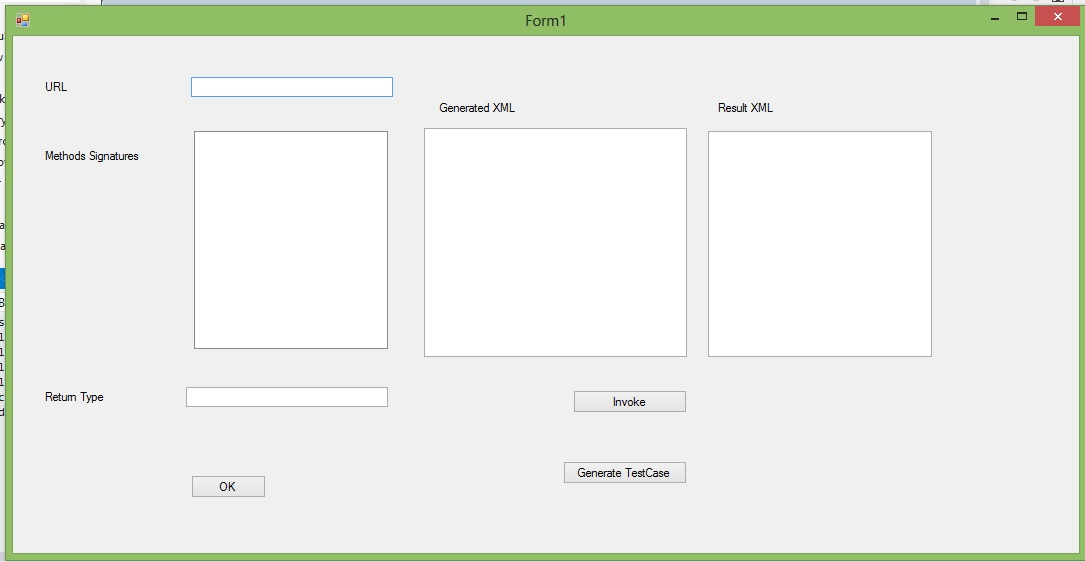
\includegraphics[width=0.7\linewidth]{MainForm}
\caption{Main Form}
\label{fig:MainForm}
		\end{figure}


	\end{block}

\end{frame}


\begin{frame}{GUI Screens}
	\begin{block}{Main Form}
		\begin{figure}
			\centering
			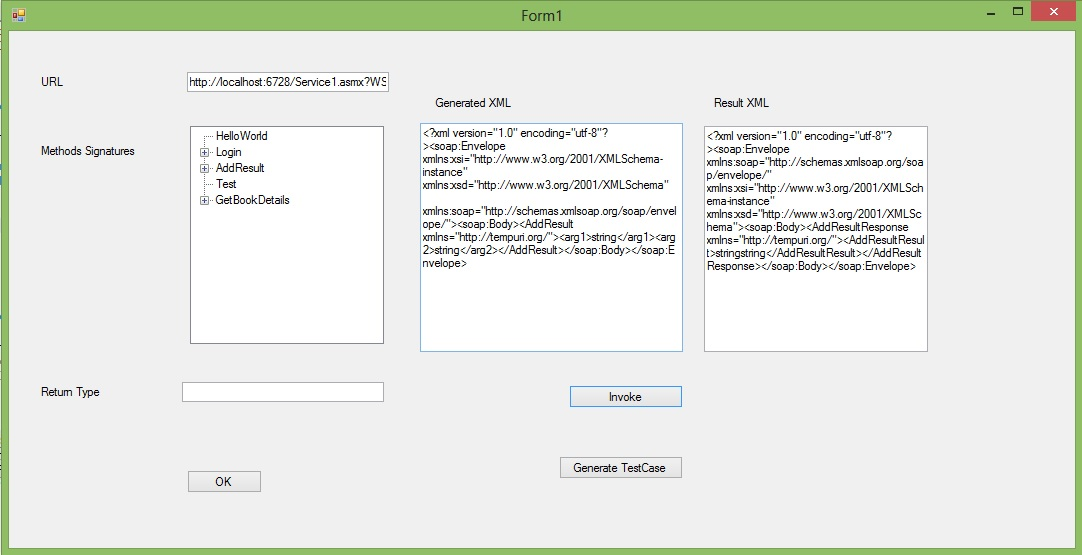
\includegraphics[width=0.7\linewidth]{MainForm1}
			\caption{Main Form}
			\label{fig:MainForm}
		\end{figure}
		
		
	\end{block}
	
\end{frame}
\begin{frame}{GUI Screens}
	\begin{block}{Test Cases}
		\begin{figure}
			\centering
			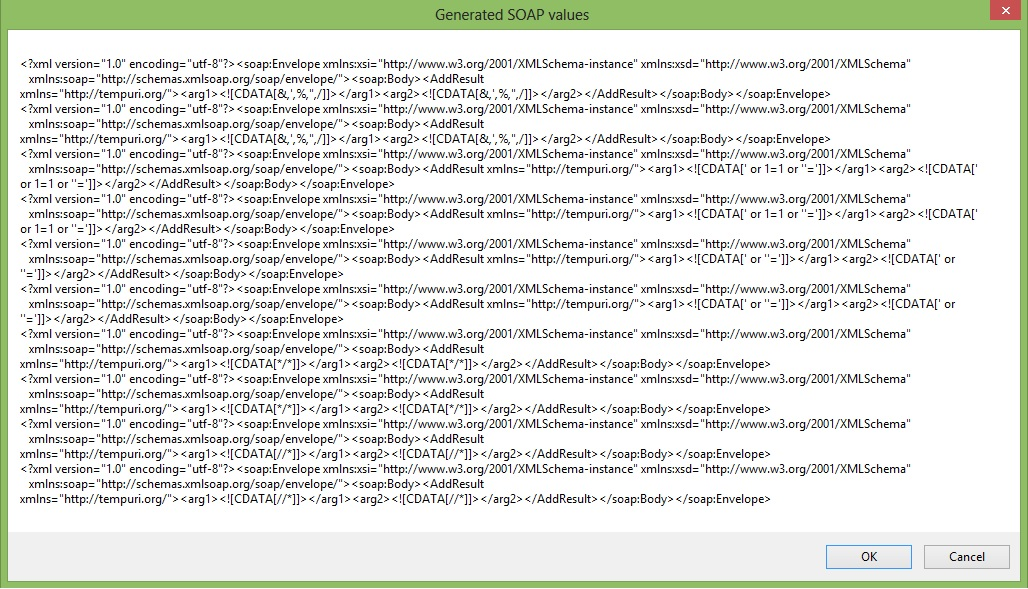
\includegraphics[width=0.7\linewidth]{TestCases}
			\caption{Main Form}
			\label{fig:Test Case Form}
		\end{figure}	
	\end{block}
\end{frame}
\begin{frame}{GUI Screens}
	\begin{block}{Results}
		\begin{figure}
			\centering
			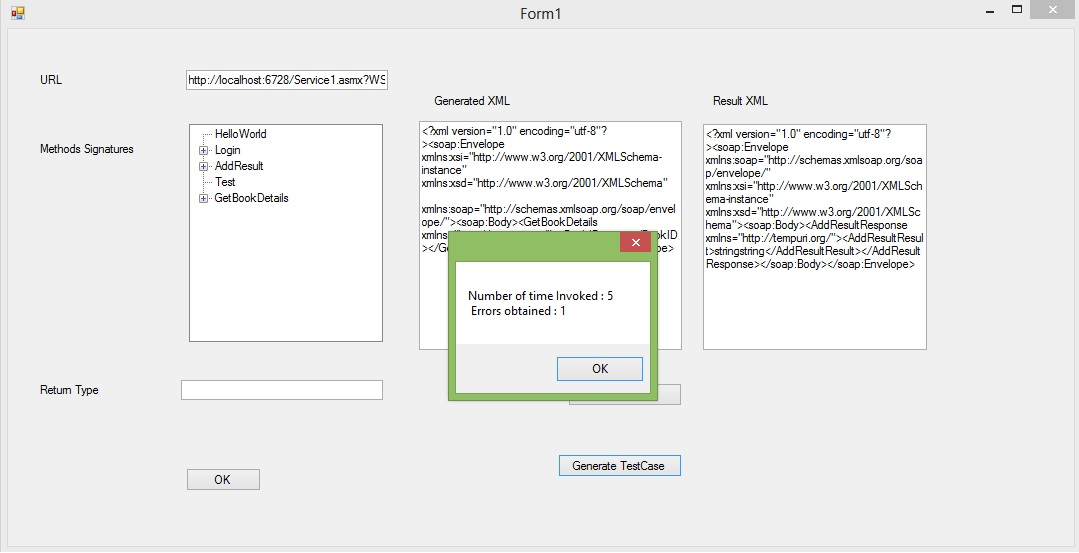
\includegraphics[width=0.7\linewidth]{Result}
			\caption{Result Form}
			\label{fig:MainForm}
		\end{figure}	
	\end{block}
\end{frame}

\section{Pending works}
\begin{frame}{To be completed}{}
	\begin{itemize}
		\item Proper analysis of output.
		\item Proper formatting of XML for display.
		\item Display output for test case invocation.
		\item Fix display issues is showing the results.
		\item Clean the code.
	\end{itemize}
\end{frame}

% Placing a * after \section means it will not show in the
% outline or table of contents.
\begin{frame}{}
	\begin{block}{}
		\begin{center}
			{\LARGE Demo}	
		\end{center}
	\end{block}
	
\end{frame}


% All of the following is optional and typically not needed. 
\begin{frame}{}
	\begin{block}{}
		\begin{center}
			{\LARGE Thank You}	
		\end{center}
	\end{block}
	
\end{frame}

\end{document}


